\documentclass{article}
\usepackage[utf8]{inputenc}
\usepackage{subfig}
\usepackage{amsmath}
\usepackage[export]{adjustbox}
\usepackage{graphicx}
\usepackage[legalpaper, landscape, margin=0.5cm]{geometry}

\thispagestyle{empty}
% \renewcommand{\thesubfigure}{\roman{subfigure}}
\begin{document}

\begin{figure}[h]
        \centering
        \subfloat[full profile]{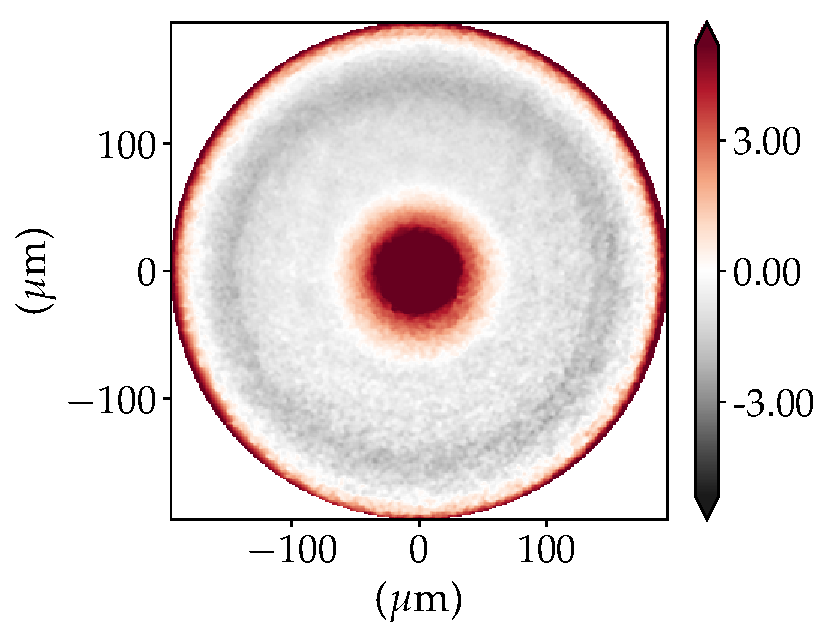
\includegraphics[height=3cm]{figures/ch06/plate_test/LSP1_V2_20x_Height_figure_errors_FF.pdf}}\hspace{0.1cm}
        \subfloat[polynomial fit]{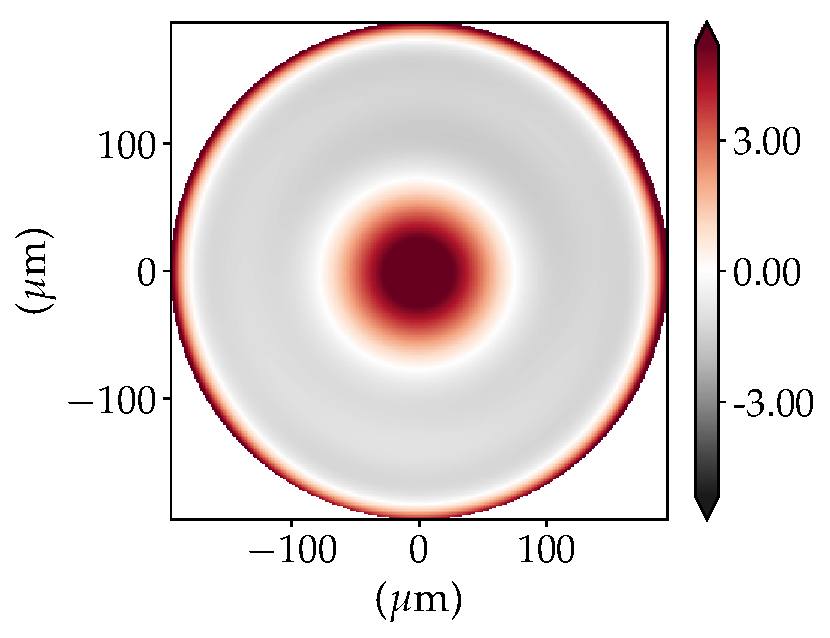
\includegraphics[height=3cm]{figures/ch06/plate_test/LSP1_V2_20x_Height_figure_errors_LF.pdf}}\hspace{0.1cm}
        \subfloat[residues]{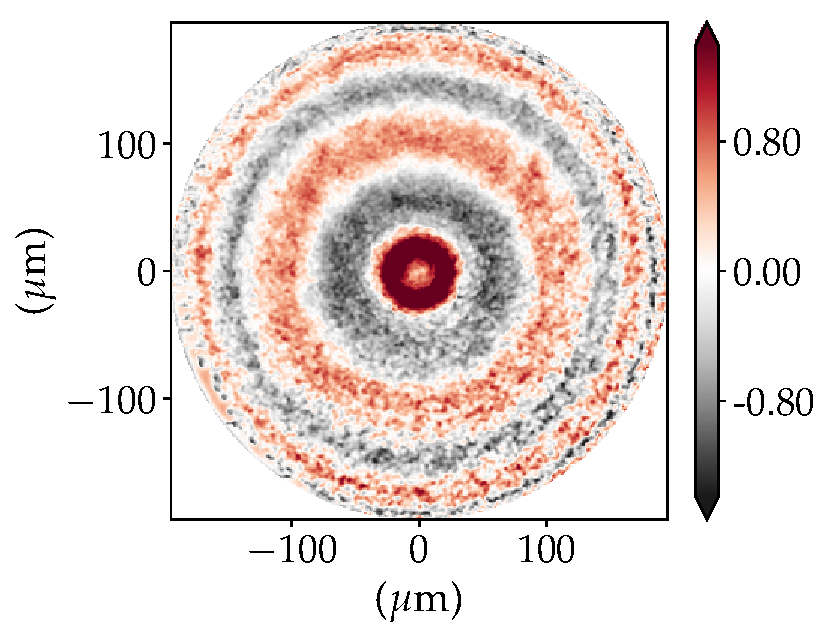
\includegraphics[height=3cm]{figures/ch06/plate_test/LSP1_V2_20x_Height_figure_errors_HF.pdf}}\\
        \subfloat[polynomial decomposition]{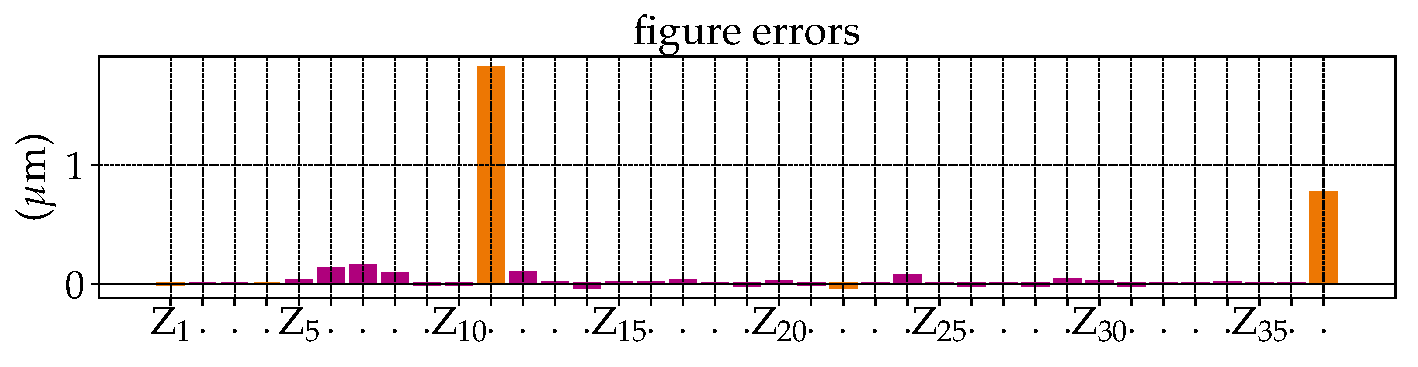
\includegraphics[height=3cm]{figures/ch06/plate_test/LSP1_V2_20x_Height_Zern_fit.pdf}}\hspace{0.1cm}
        \subfloat[azimuthally averaged profile]{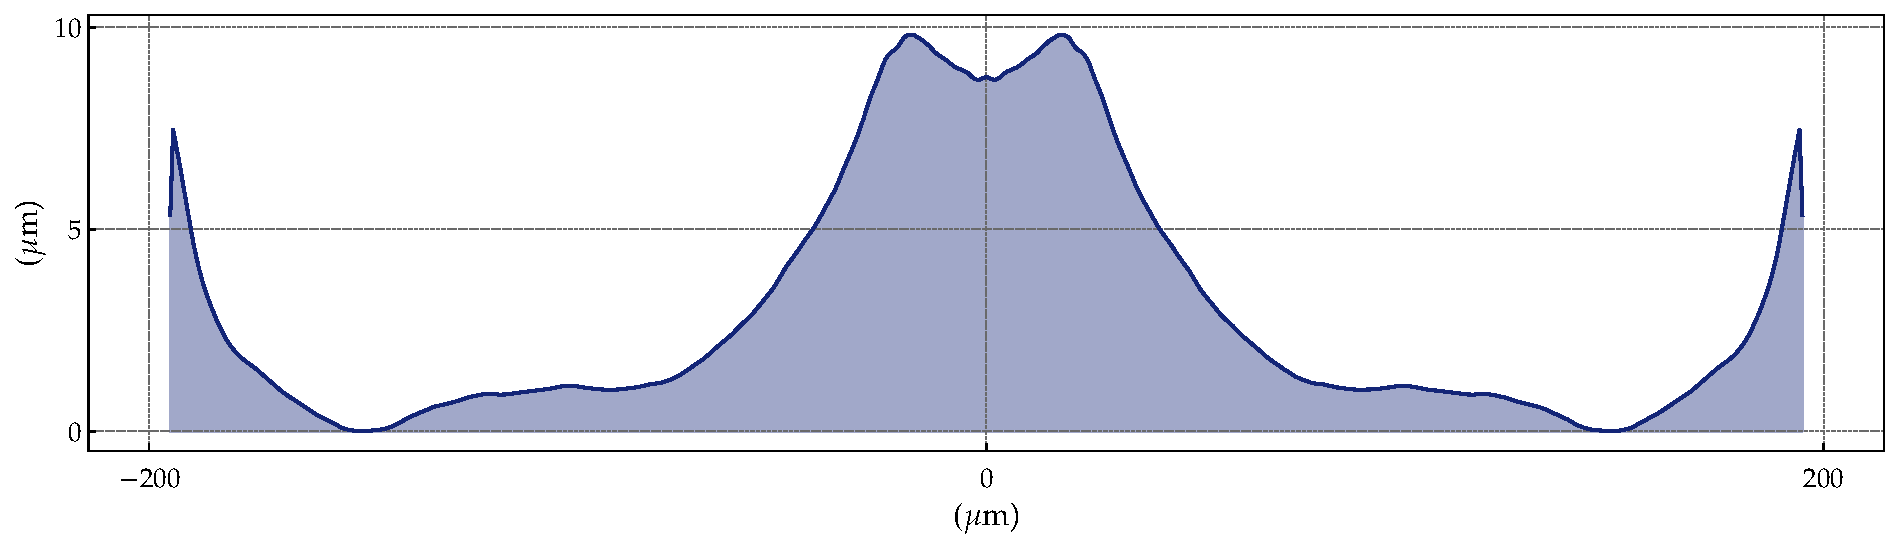
\includegraphics[height=2.6cm]{figures/ch06/plate_test/LSP1_V2_20x_Height_correction_plate_cut_2.pdf}}
\end{figure}
\end{document}